\chapter{Revisão bibliográfica}
\label{chap:revisao}

\section{Arquiteturas Multi-Agentes para Otimização}
\citeonline{silva2018} faz uma detalhada revisão da literatura apresentando 25 arquiteturas de software voltadas para otimização. 
A autora apresenta os trabalhos em duas categorias, a saber: \textit{frameworks} para otimização que utilizam metaheurísticas e \textit{frameworks} multi-agentes que utilizam metaheurísticas. Entre essas duas principais categorias, são analisadas características gerais e avançadas, características multi-agentes, e os recursos ao processo de otimização. 

O que se propõe neste trabalho é desenvolver uma arquitetura de software multi-agente, distribuída, baseada no modelo de atores, e escalável. Neste sentido, há que se comparar este trabalho com trabalhos semelhantes apresentados na literatura. Dos 25 trabalhos apresentados por \citeonline{silva2018}, foram selecionados aqueles que são categorizados como um sistema distribuído em suas características avançadas, e que são sistemas multi-agentes.

Deste modo, as próximas subseções apresentam as arquiteturas AgE, CMA, JABAT, MACS e MANGO, com suas principais características. Adiante também haverá uma apresentação da arquitetura D-Optimas, objeto de estudo do presente trabalho, a seção seguinte fará um comparativo dos trabalhos apresentados anteriormente e como a versão atual do D-Optimas se destaca dentre as outras.

\subsection{AgE}
AgE, abreviatura para \textit{Agent Evolution}, foi proposto por \citeonline{cetnarowicz1996application} e é definido como uma plataforma baseada em componentes, configurável, para a resolução de diferentes problemas \cite{piketak2009functional}. O autor apresenta um formalismo matemático para definir um modelo baseado em agentes e descreve como esse formalismo pode ser implementado utilizando componentes de software reutilizáveis. A implementação é feita em Java, baseado no \textit{Pico Container}\footnote{http://picocontainer.com}, um \textit{middleware} para inversão de controle e injeção de dependências. O autor defende que é possível utilizar várias técnicas de otimização \cite{piketak2013agent}, entretanto a única implementação concreta do \textit{framework} é baseada em algoritmos genéticos e sistemas multi-agentes evolucionários \cite{kisiel2004agent}. Há outras implementações do AgE em diferentes linguagens, mas não foram encontrados trabalhos que apresentem resultados experimentais, ou que demostrem o funcionamento ou vantagens do modelo. 

\subsection{CMA}
\citeonline{malek2009} propôs o Algoritmo para Colaboração de Meta-heurísticas (CMA). Este é um \textit{framework} para resolução de problemas de otimização combinatória. O sistema conta com quatro tipos diferentes de agentes. O primeiro deles, são agentes do tipo Problema, responsável por receber os dados de entrada do usuário e iniciar o processo de otimização. Há um agente responsável por manter o conjunto de soluções encontradas até o momento e fornecer essas soluções para os agentes otimizadores. A comunicação entre os agentes acontece de maneira indireta através desse agente chamado \textit{SolutionPool}, não havendo de fato uma colaboração efetiva entre os agentes. Os otimizadores encapsulam as meta-heurísticas e, por fim, há um agente consultor que é responsável por calibrar e fornecer os parâmetros para cada agente. O autor apresenta resultados para algumas instâncias do Problema do Caixeiro Viajante \cite{malek2010}, mas sem uma análise estatística aprofundada, exibindo somente o melhor valor encontrado para cada instância. 

\subsection{JABAT}
JABAT é um sistema multi-agentes no qual os agentes colaboram para gerar soluções de problemas de otimização combinatória. Ele é baseado no A-Teams e implementando com o suporte da biblioteca \textbf{JADE} (\textit{Java Agent Development Framework}). Foi proposto inicialmente por \citeonline{jedrzejowicz2006} e a última atualização do trabalho, feita por \citeonline{barbucha2010}, apresenta duas novas versões da arquitetura: eJABAT que oferece uma interface Web e a cJABAT que incluí um mecanismo de aprendizagem por reforço positivo. Estas novas versões, de acordo com o autor, são escaláveis, portáveis e em conformidade com a \textbf{FIPA} (\textit{Foundation of Intelligent Physical Agents}). 

O autor apresenta também os problemas resolvidos pela arquitetura JABAT, a saber: \textit{Resource Constrained Project Scheduling} (RCPSP) com e sem restrição de tempo, \textit{Euclidean Planar TSP}, \textit{Clustering} e distribuído e não distribuído, \textit{Vehicle Routing Problem}, e \textit{Data Reduction Problem} distribuído e não distribuído. Apesar da argumentação de que a arquitetura é genérica, cada problema é apresentado com um conjunto específico de heurísticas para resolvê-lo. O autor não deixa claro se é possível mudar a estratégia de solução de cada problema. 

A arquitetura conta com um mecanismo de aprendizagem por reforço, que nesta configuração passa a funcionar de maneira síncrona. O mecanismo atribui pesos a cada agente que são atualizados à medida que cada um deles produz uma solução. Os pesos são utilizados em um sorteio ponderado para escolher que agente executará a cada instante de tempo. Entretanto, a arquitetura não é preparada para solucionar problemas multi-objetivo. 

\subsection{MACS}
\citeonline{martin2016} propôs um sistema multi-agente para busca cooperativa (do inglês \textit{Multi-Agent Cooperative Search}, MACS) para a resolução de problemas de roteamento e fluxo. O sistema foi baseado no \textit{JADE} e possui somente dois tipos de agente, denominados inicializador e agente meta-heurístico. O primeiro tipo é responsável por ler os dados do problema e convertê-los numa representação compatível com o protocolo de comunicação dos agentes  do segundo tipo, que encapsulam um par de meta-heurística/busca local. A colaboração acontece entre os agentes através de um protocolo de comunicação denominado conversação. O autor compara os resultados utilizando um, quatro, oito e dezesseis agentes colaborando, e foi possível perceber diferença significativa (95\% de confiança) no resultado da busca sempre que se dobra o número de agentes. Além disso, os resultados obtidos foram tão bons quanto os da literatura, sem a necessidade de ajuste de parâmetros. Entretanto, foram utilizados somente as heurísticas RandNEH \cite{juan2010b} e RandCWS \cite{juan2010a}.

\subsection{MANGO}
O Ambiente Multi-Agente para Otimização Global (MANGO) apresentado por \citeonline{kerccelli2008} é uma arquitetura baseada também na plataforma JADE. Cada agente encapsula uma meta-heurística e pode se comunicar com outros agentes, compartilhando e solicitando soluções, ou informando sobre áreas do espaço de busca que são propícias para exploração. A comunicação entre os agentes acontece de maneira assíncrona e não-determinística através de troca de mensagens. A implementação da arquitetura é fortemente acoplada ao problema de otimização e só possui a heurística EM (\textit{Eletromagnetism-like Mechanism}, Mecanismo Eletromagnético em português) \cite{birbil2003}. O autor apresenta apenas uma execução para ilustrar o funcionamento da arquitetura, não apresentando um procedimento experimental planejado.


\subsection{AMAM}
O \textit{framework} AMAM, proposto inicialmente por \citeonline{silva2007} é um MAS composto por 5 tipos de agentes, a saber: os construtores, agentes de busca local, agentes que encapsulam meta-heurísticas, o agente coordenador e o analisador de soluções. Os três primeiros agentes são responsáveis por explorar o espaço de busca, enquanto o coordenador, que centraliza a troca de mensagens, é responsável por intermediar a comunicação entre os outros agentes. A primeira versão da AMAM foi proposta por \citeonline{oliveira2008} e estendida por \citeonline{fernandes2009}, que a equipou com uma memória adaptativa compartilhada. Nesta versão, a comunicação entre os agentes se dá por meio de uma área de memória compartilhada que mantém as melhores soluções a arquitetura em um dado momento. O acesso à essa área pelos agentes é feito de maneira síncrona.  

A versão mais recente do AMAM abandonou o conceito de agente coordenador, se alinhando a melhor prática de modelagem de sistemas multi-agentes, em que a independência dos agentes é um princípio importante. Nesta versão, os agentes são dotados de uma memória de aprendizagem por reforço \cite{silva2015}. Os resultados neste trabalho indicam que há diferença significativa nos resultados encontrados pela arquitetura quando há  cooperação entre os agentes, mesmo em uma simulação de pequeno porte, com somente quatro agentes.

O \textit{framework} AMAM e a arquitetura BIMASCO tiveram a mesma origem, como relata a seção a seguir. A principal diferença entre os dois trabalhos é que a AMAM não faz uso de mecanismos de programação distribuída ou paralela e, em suas primeiras versões, utiliza um modelo de comunicação determinístico. Além disso, a arquitetura BIMASCO já suportava na sua última versão, diferentes tipos de problemas de otimização, enquanto a AMAM  oferece suporte somente para problemas de otimização combinatória.

\section{Histórico da Arquitetura D-Optimas}
\label{sec:histBimasco}

Um projeto mais recente,no qual o presente trabalho se baseia, é a arquitetura D-Optimas. Essa arquitetura foi apresentada por \citeonline{pacheco}, mas é fundada num projeto mais antigo, chamado BIMASCO, que possui um longo histórico e uma bibliografia densa. Esta secção é dedicada a fazer uma pequena revisão do projeto, desde sua origem no trabalho de \citeonline{saliba2010}, passando pelos trabalhos de \citeonline{denise2014} e \citeonline{marcus2015}, até a sua transformação em uma arquitetura distribuída para solução de problemas de otimização. Serão apresentados os principais conceitos que compõe a arquitetura, os resultados obtidos em cada uma de suas versões, e as suas eventuais falhas conceituais.

A arquitetura BIMASCO (\textit{Bio Inspired Multi Agent System for Combinatorial Optimization} foi primeiramente apresentada por \citeonline{saliba2010} como uma completa reconcepção da arquitetura AMAM, segundo o próprio autor. Foi desenvolvida no Laboratório de Sistemas Inteligentes do CEFET-MG e a justificativa para a sua criação foi baseada no fato de que a AMAM, como já apresentado na seção anterior, feria alguns princípios da modelagem de sistemas multi-agentes, principalmente o princípio da autonomia, prevendo em seu modelo um agente controlador que determinava o comportamento dos demais agentes. O objetivo do trabalho àquele momento foi implementar um sistema multi-agente que funcionasse por troca de mensagens assíncrona, de modo que os agentes pudessem interagir entre si e com o espaço de busca, tomando decisões de maneira autônoma, funcionando como um sistema auto-organizável \cite{saliba2010}. 

Para o desenvolvimento do seu trabalho o autor se baseou numa outra arquitetura de software, essa voltada para a simulação de vida artificial, chamada ARTÍFICE. Esse projeto foi desenvolvido por cerca de 15 anos no mesmo laboratório. Seu objetivo era modelar, construir e simular criaturas artificiais com sistema nervoso central, e era fortemente fundamentado em conceitos biológicos e da cognição situada. Essas criaturas deviam ser capazes de aprender, se adaptar, bem como viver em um mundo artificial \cite{santos2003}. Uma lista não exaustiva dos principais trabalhos que compõe a arquitetura ARTÍFICE são: \citeonline{campos2006}, quem propôs a primeira implementação, \citeonline{silva2008}, que apresentou um mecanismo de aprendizagem por reforço e \citeonline{mapa2009}, que adicionou ao software um sistema de memória episódica. 
Destes projetos, o BIMASCO herda sua característica mais inovadora à época, seu caráter bio-inspirado. Ainda hoje, olhando para a literatura mais recente, em especial a revisão feita por \citeonline{silva2018} não se tem relato de nenhum trabalho que dialogue com áreas do conhecimento tão diversas. 

Feita esta pequena introdução sobre o histórico do projeto, passemos às contribuições da primeira implementação do BIMASCO proposta por \citeonline{saliba2010}. Além da inovação de um sistema multi-agente bio-inspirado para otimização, baseado em programação \textit{multi-threading}, que permitia escalar o sistema verticalmente\footnote{Entende-se aqui por escalabilidade vertical a capacidade de aumentar o sistema adicionando mais recursos na mesma máquina. Mais adiante será mencionado o conceito de escalabilidade horizontal que é a capacidade de um sistema crescer a medida que se adicionam mais máquinas à configuração, como em um \textit{cluster}, por exemplo.}, o autor apresenta a arquitetura como uma metáfora biológica composta de 3 entidades: agentes, regiões e o mundo. O \textbf{mundo artificial} é o espaço de busca, composto das \textbf{soluções} de um problema de otimização, que podem ser agrupadas em \textbf{regiões} de interesse. Essas regiões não são necessariamente estáticas, podendo contrair, expandir, particionar e se unir a outras regiões. A \autoref{fig:bimasco_saliba} ilustra didaticamente o sistema proposto pelo autor. 

\begin{figure}
    \centering
    \caption{Representação gráfica do projeto BIMASCO, onde é possível distinguir os agentes, regiões, soluções no espaço de busca, bem como os possíveis movimentos de um agente}
    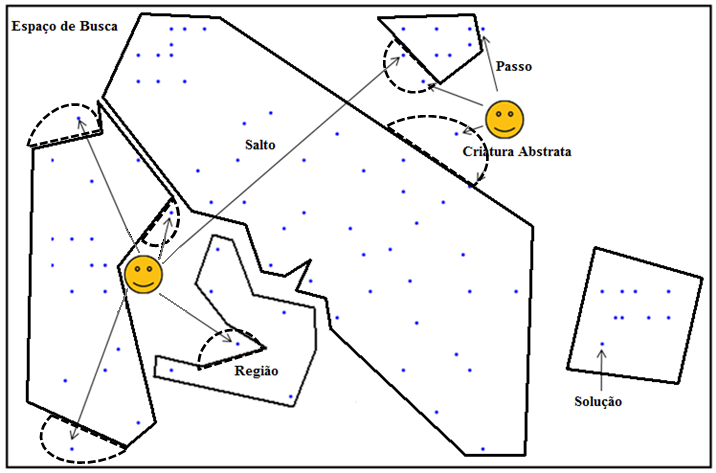
\includegraphics[scale=0.45]{imagens/bimasco-saliba.png}
    \fonte{\citeonline{saliba2010}}
    \label{fig:bimasco_saliba}
\end{figure}


Neste ponto é necessário ressaltar que apesar do autor prever a divisão do espaço em regiões, e introduzir um comportamento básico para elas, ele não entra em detalhes do seu funcionamento e também não as implementa.

Os \textbf{agentes} são formados pela união de vários componentes. Entre os principais estão os mecanismos de aprendizagem, componentes emocionais, efetores e sensores. Além disso, encapsulam as heurísticas e meta-heurísticas e interagem com esse espaço de busca, produzindo e consumindo soluções do mundo, aprendendo a buscar melhores soluções. Cada componente do agente executava em uma \textit{thread} separada, que se comunicavam por troca de mensagens, por meio de uma área de memória compartilhada, chamada de \textit{Interoceptive Pool}. A \autoref{fig:interoceptive_pool_saliba} ilustra os diversos componentes que compõe o agente, incluindo os sensores, efetores, componentes do sistema nervoso artificial, bem como a comunicação entre eles por meio de memória compartilhada.

\begin{figure}
    \centering
    \caption{Esquema dos componentes internos do agente, os estímulos, ou mensagens que eles trocam entre si, e o \textit{Interoceptive Pool}, memória compartilhada utilizada para a troca de mensagens}
    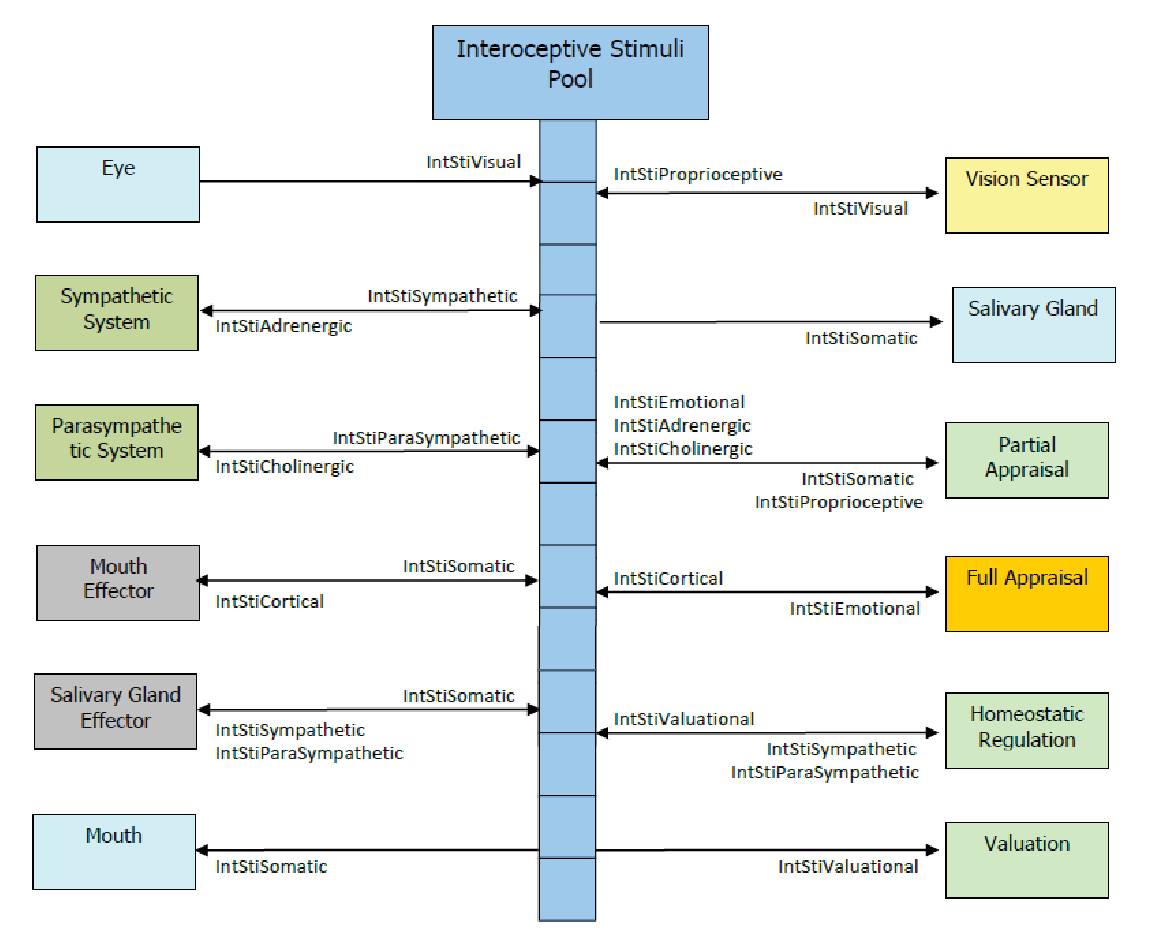
\includegraphics[scale=0.6]{imagens/interoceptive-pool-saliba.eps}
    \fonte{\citeonline{saliba2010}}
    \label{fig:interoceptive_pool_saliba}
\end{figure}

O objetivo é que os agentes aprendam a encontrar boas soluções para um problema de otimização baseado nessa interação e na colaboração entre eles. A interação com o espaço de busca acontece também por meio de troca de mensagens,  baseada em compartilhamento de estado, por meio do \textit{Environmental Pool}. A \autoref{fig:bimasco_env_pool} ilustra o funcionamento do \textit{Environmental Pool}, que é basicamente uma lista compartilhada onde agentes e regiões podem colocar mensagens endereçadas a outras entidades, bem como consultar periodicamente se há mensagens endereçadas para si.

\begin{figure}
    \centering
    \caption{Mensagenes trocadas entre agentes e regiões através do \textit{Environmental Pool}.}
    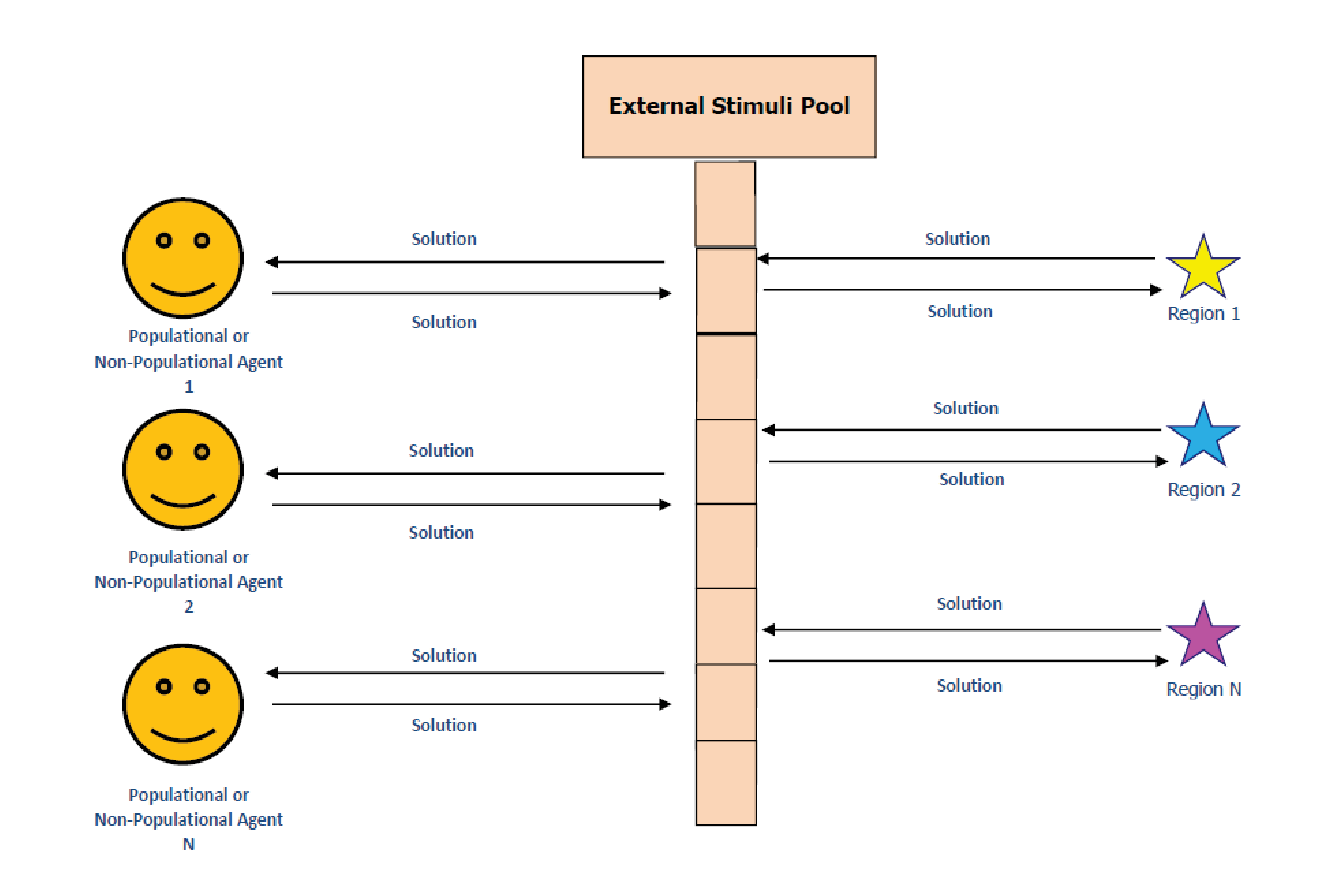
\includegraphics[scale=0.5]{imagens/external-pool-saliba.eps}
    \fonte{\citeonline{saliba2010}}
    \label{fig:bimasco_env_pool}
\end{figure}

Os agentes podem ser divididos em construtores, populacionais e não-populacionais, baseado no funcionamento de cada um e em suas interações com o espaço de busca. Um agente construtor, por exemplo, não precisa consumir nenhuma solução inicial do mundo, pois constrói uma solução, elemento a elemento, baseado em alguma estratégia, que pode ser gulosa ou randômica. Um agente populacional encapsula uma estratégia de busca baseada em populações, \textit{e.g.}, um algoritmo genético, e por isso necessita de um conjunto inicial de soluções para funcionar. Assim, o agente busca soluções iniciais no espaço de busca, processa e entrega um conjunto melhorado de soluções ao mundo. Agentes não-populacionais são aqueles que realizam buscas locais, e necessitam de uma solução para iniciar a busca, produzindo uma solução que pode ser um ótimo local, ou um ótimo global. 

Nesta primeira versão da arquitetura estavam presentes algumas estratégias de busca conhecidas da literatura, são elas: a heurística construtiva GRASP (\textit{Greedy Randomized Adaptive Search Procedure}), os métodos de busca local ILS (\textit{Iterated Local Search}) e VNS (\textit{Variable Neighborhood Search}) e a meta-heurística populacional GA (\textit{Genetic Algorithm}). Para avaliar o funcionamento da sua arquitetura, \citeonline{saliba2010} executou alguns experimentos com instâncias do Problema de Roteamento de Veículos com Janela de Tempo (PRVJT), propostas por \citeonline{solomon1987}, e compara os seus resultados com os da arquitetura AMAM. Entretanto, ele não apresenta um procedimento experimental adequado para um sistema não-determinístico, como é o BIMASCO, e muito menos uma análise estatística rigorosa, prejudicando uma comparação entre as arquiteturas. 

Apesar de \citeonline{saliba2010} ter projetado o BIMASCO para ser facilmente extensível e flexível tanto para os métodos de busca quanto para os problemas, foi somente no trabalho de \citeonline{denise2014} que a arquitetura foi estendida para que as heurísticas fossem completamente independentes da representação e dados dos problemas. Para tanto, a autora tornou as soluções genéricas quanto ao tipo de dado, podendo ele ser booleano, inteiro ou real. Também criou artefatos de software para abstrair as estratégias que atuam sobre as soluções e que são comuns a vários algoritmos de busca. Esses artefatos foram nomeados \textbf{movimentos}, que consistem na alteração de uma posição do vetor no espaço de objetivos, levando a solução para um vizinho próximo, e  \textbf{modificadores}, que podem ser vistos como um conjunto de movimentos. Um movimento ou um modificador pode ser aplicado a uma ou mais soluções, e foram implementados para as principais heurísticas e para os tipos de dados propostos. A autora deixa claro que "[...]  os modificadores são totalmente dependentes do tipo de
representação do problema e não do problema em questão" \cite{denise2014}. 

Nesta versão do BIMASCO novos problemas foram adicionados à arquitetura, a saber: o problema da otimização irrestrita de função real,  da diversidade máxima, da mochila e o problema da partição binária. Foi adicionada a heurística \textit{Simulated Anealing} e as heurísticas existentes foram adaptadas para funcionarem de maneira independente da representação das soluções, utilizando somente os movimentos e modificadores propostos. Em seguida, foram apresentados três conjuntos de experimentos para validar a generalização da arquitetura executando diferentes combinações de problemas e heurísticas, bem como o correto funcionamento das heurísticas. A arquitetura alcançou bons resultados para a maioria dos problemas, apesar do efeito dos mecanismos de aprendizagem não ter sido avaliado, e a implementação dos comportamentos para as regiões foi elencada somente na seção de trabalhos futuros. 

Dando prosseguimento no trabalho de \citeonline{denise2014}, \citeonline{marcus2015} simplificou a arquitetura, removendo a maioria dos componentes herdados da arquitetura ARTÍFICE que oneravam a simulação, tornando-a mais lenta e menos competitiva que outras arquiteturas. Deste modo, o autor propõe um mecanismo simplificado baseado em aprendizagem  por reforço, um protocolo de comunicação entre os agentes, e uma primeira implementação da dinâmica das regiões. Nesta nova versão, os agentes passam a ser compostos somente de 3 \textit{threads}: um componente sensor, efetor e o \textit{Evaluator}. Por meio do componente sensor, os agentes podem solicitar soluções a outros agentes e às regiões, com uma probabilidade associada. Essa probabilidade é alterada a medida que o agente interage com o mundo e produz soluções melhores do que as produzidas anteriormente. Essas soluções são avaliadas pelo \textit{Evaluator}, que altera as probabilidades na memória do agente. 

Para escolher, dentre os agentes e regiões na memória, de qual solicitar soluções, o algoritmo funciona basicamente em duas etapas. Inicialmente, ele faz uma roleta entre todos os agentes e reserva uma fatia dessa roleta para as regiões. Caso algum agente seja sorteado, é enviado uma mensagem diretamente para ele. Mas caso a escolha recaia sobre as regiões, é feita uma nova roleta entre as regiões, e o agente pede soluções para a região escolhida. O agente utiliza as soluções recebidas para executar a meta-heurística que encapsula e produzir novas soluções, que retornam para o mundo. O componente efetor é responsável por enviar essas soluções produzidas para uma região. Entretanto, \citeonline{marcus2015} não dá detalhes sobre como um agente escolhe para qual região enviar essas novas soluções. 

A estratégia proposta para a fusão e fissão das regiões ficou baseada na análise da variância e covariância dos valores de função objetivo dos conjuntos de soluções que formam as regiões. Para se dividir, uma região verifica se a variância da função objetivo está acima de um limiar que é dado como parâmetro no arquivo de configuração da simulação. Se a $\sigma^{2}$ for maior que este parâmetro, a  região se particiona em 3 novas regiões contendo as soluções com valor de função objetivo que estavam abaixo de $\mu - \sigma$, entre $\mu - \sigma$ e $\mu + \sigma$ e as que estavam acima de $\mu + \sigma$. Para duas regiões fazerem fusão, a covariância entre as duas tem de ser maior que um limiar, que também é um parâmetro da configuração da arquitetura. É importante observar que o autor não mostra detalhadamente como essa analise é feita. Por exemplo, a fórmula da covariância entre duas amostras $X$ e $Y$ de tamanho $N$ com médias $\overline{X}$ e $\overline{Y}$ pode ser escrita da seguinte maneira:
\begin{equation}
\label{eq:cov}
    cov(X,Y) = \sum_{i=1}^{i<N}\frac{(x_i - \overline{X})(y_i - \overline{Y})}{N - 1} 
\end{equation} 
Aplicando a \autoref{eq:cov} ao contexto da fusão entre duas regiões, seria necessário que ambas tivessem o mesmo número $N$ de soluções. Entretanto, pela característica estocástica do sistema, muito raramente duas regiões terão o mesmo número de soluções. Esse caso de borda não foi abordado na modelagem do autor, muito menos nos experimentos realizados. 

Neste trabalho foram executadas 5 baterias de experimentos dos quais 4 estavam voltados para avaliar o desempenho da arquitetura com e sem colaboração entre os agentes (permitindo ou não que os agentes troquem soluções) e 1 voltado para avaliar o efeito de utilizar uma ou mais regiões na simulação, alterando somente os limiares de fusão e fissão. Na maioria dos experimentos foi observado que a interação entre os agentes e a aprendizagem favorecem a busca por melhores soluções. No entanto, não foi possível tirar alguma conclusão sobre o efeito da separação do espaço em regiões para o funcionamento da arquitetura.

A falta de experimentos em larga escala com a arquitetura BIMASCO motivou \citeonline{pacheco} a propor uma nova implementação da arquitetura, desta vez baseada num modelo de concorrência mais moderno, denominado modelo de atores. Proposto inicialmente por \citeonline{hewitt1973}, o modelo de atores se contrapõe ao modelo de concorrência por \textit{threads} e compartilhamento de estado. Os atores, unidades básicas de computação, não compartilham o estado interno e se comunicam somente por meio de troca de mensagens assíncronas. O autor utilizou como ferramenta o \textit{framework Akka}\footnote{https://akka.io/}, uma implementação do modelo de atores para linguagens baseadas na JVM, como o Java. 

A mudança de paradigma oferece à arquitetura remodelada a vantagem de poder escalar horizontalmente, como um sistema distribuído, o que inclusive leva à mudança do nome do projeto, que deixa de se chamar BIMASCO e passa a se chamar D-Optimas. Os agentes e regiões também foram reduzidos a um único ator que executa a regra de negócio principal, mas sem perderem as suas funcionalidades descritas nos trabalhos anteriores. 

A \autoref{fig:d_optimas_pacheco} ilustra a hierarquia de atores proposta por \citeonline{pacheco}. O ator \textit{/user} faz parte do \textit{toolkit Akka} e supervisiona todos os atores criados pelo programa, os atores \textit{/agents} e \textit{/regions} criam, supervisionam e finalizam a execução de agentes e regiões, respectivamente. O ator \textit{/reaper} é o responsável por finalizar a simulação quando atingido o critério de parada. Uma maneira possível de executar essa arquitetura em um \textit{cluster}\footnote{No contexto da computação distribuída, um \textit{cluster} nada mais é do que um conjunto de computadores conectados através de uma rede, os quais podem ser chamados de membros, nós, \textit{workers}, \textit{slaves}, a depender do autor. O presente trabalho utiliza o termo nó, por não haver qualquer distinção entre o papel dos computadores em si. } seria alocar o ator \textit{/agents} em uma máquina com o endereço \textit{192.168.0.1}, e o \textit{/regions} no computador endereçado no IP \textit{192.168.0.2}, ambos na porta \textit{2551}. Para o agente \textit{a1} se comunicar com a região \textit{r1} é necessário que ele saiba o endereço completo do agente, que seria \textit{akka://192.168.0.2:2551/user/regions/r1}.

\begin{figure}
    \centering
    \caption{Hierarquia de atores proposta para a arquitetura D-Optimas.}
    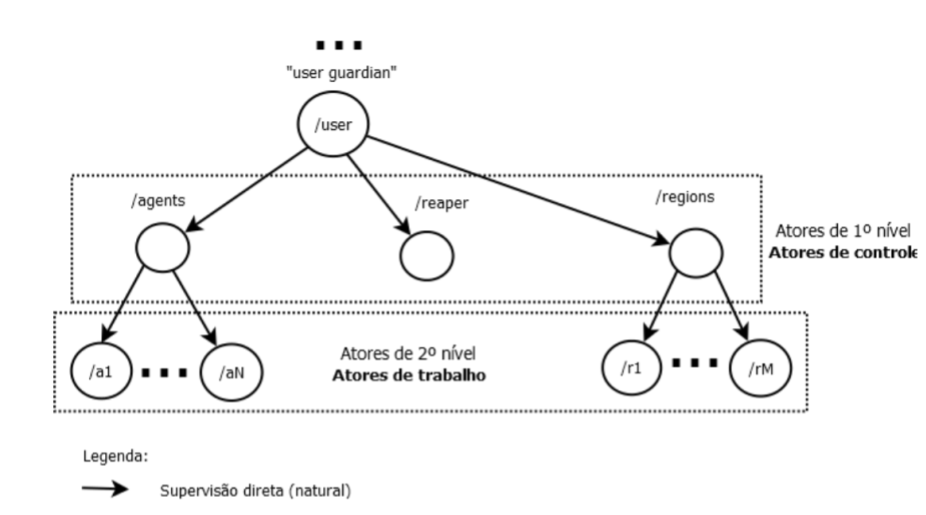
\includegraphics[scale=0.4]{imagens/d-optimas-pacheco.png}
    \fonte{\citeonline{pacheco}}
    \label{fig:d_optimas_pacheco}
\end{figure}

O autor apresenta dois experimentos para avaliar o resultado da mudança: o primeiro, para verificar a corretude do sistema e certificar de que a mudança de paradigma não alterou nenhuma funcionalidade até aqui desenvolvida, e um segundo que avaliou a escalabilidade da arquitetura, coletando dados de 30 execuções com mais de 1000 agentes. Entretanto, o segundo e principal experimento não avaliou o funcionamento da arquitetura em mais de 2 nós, não exibindo nenhum dado sobre a escalabilidade horizontal do sistema.

\section{Considerações Finais}
O presente capítulo se dedicou a fazer uma revisão da literatura de arquiteturas multi-agentes para otimização. Foram apresentadas alguns trabalhos que compartilham características importantes, baseado principalmente na revisão mais recente realizada por \citeonline{silva2018}. Entre essas arquiteturas, foi apresentada também a arquitetura AMAM, proposta por \citeonline{silva2019} e por fim, a arquitetura D-Optimas. As suas principais características, resultado de diversas contribuições ao longo dos últimos 10 anos, foram exploradas, bem como suas eventuais deficiências, que se convertem em boas oportunidades de trabalho. O capitulo seguinte apresenta os esforços que foram feitos no presente trabalho para reparar essas deficiências e estender o projeto. 